% AI-ML Systems 2026 — Research Track Submission
% Double-blind, double-column IEEE format
% Page limit: 8 pages + references (no appendix)

\documentclass[conference]{IEEEtran}

\usepackage{times}
\usepackage{url}
\usepackage[hidelinks]{hyperref}
\usepackage[utf8]{inputenc}
\usepackage[small]{caption}
\usepackage{graphicx}
\usepackage{amsmath}
\usepackage{booktabs}
\usepackage{tabularx}
\usepackage{multirow}
\usepackage[table]{xcolor}
\usepackage{pgfplots}
\usepackage{tikz}
\pgfplotsset{compat=1.18}
\usepackage{colortbl}
\usepackage{cite}

% ---- colour palette (reused from original) ----
\definecolor{bestgreen}{RGB}{0,140,60}
\definecolor{worstred}{RGB}{185,30,30}
\definecolor{dravidianrow}{RGB}{255,245,220}
\definecolor{colDrav}{HTML}{d46030}
\definecolor{colIAL}{HTML}{5ba4cf}
\definecolor{colIAH}{HTML}{1b4e96}
\definecolor{axiscol}{HTML}{bbbbbb}
\definecolor{gridcol}{HTML}{eeeeee}
\definecolor{labelcol}{HTML}{333333}
\definecolor{subtlecol}{HTML}{555555}

\newcommand{\best}[1]{\textcolor{bestgreen}{\textbf{#1}}}
\newcommand{\worst}[1]{\textcolor{worstred}{\textbf{#1}}}

\urlstyle{same}

% ---- double-blind: author block intentionally omitted ----
\title{Trustworthiness of LLMs in Cross-Lingual Clinical Summarization:\\
An Empirical Study on Indian Languages}

\begin{document}

\maketitle

% ==================================================================
\begin{abstract}
Clinical AI systems are overwhelmingly benchmarked in English, yet
over a billion speakers of Indian languages rely on healthcare systems
where consultations occur in diverse regional languages.
We study whether open-source LLMs can generate trustworthy English
clinical summaries directly from multilingual doctor--patient dialogues.
We evaluate two 7B-parameter models (Mistral-7B and Qwen2.5-7B)
across ten typologically diverse Indian languages under four settings:
zero-shot prompting, few-shot prompting ($k{=}1$), translation-then-summarize
(via IndicTrans2), and LoRA-based supervised fine-tuning.
Key findings: few-shot prompting \emph{degrades} performance in 8 of
10 language pairs; translation helps Indo-Aryan languages but harms
Dravidian languages; clinical safety scores remain below 3.0/5.0 across
all conditions; and supervised fine-tuning reduces hallucination rates
from $\sim$42\% to $\sim$10\% while nearly eliminating cross-lingual
performance disparities.
We further contribute a systematic eight-category Clinical Error Taxonomy
characterising failure modes by method and language family.
\end{abstract}

% ==================================================================
\section{Introduction}

Accurate clinical documentation is a cornerstone of modern healthcare.
Doctor--patient consultations contain symptoms, diagnostic reasoning,
medication histories, and psycho-social context that are vital for continuity
of care, yet much of this content is never reliably captured in structured
records. In India alone, primary healthcare workers conduct hundreds of millions
of consultations annually across a population speaking 22 constitutionally
scheduled languages spanning four major language families~\cite{gala2023indictrans2}.
Errors of omission in clinical notes are a well-documented source of adverse
patient outcomes~\cite{clusmann2023future}.

Instruction-tuned LLMs achieve competitive performance on English clinical
summarization benchmarks~\cite{tang2023gersteinlab,abacha2023overview},
but the overwhelming majority of clinical NLP research targets
high-resource languages, leaving a vast multilingual documentation need
unaddressed. For Indian languages — ranging from well-resourced Indo-Aryan
languages (Hindi, Bengali) to morphologically complex Dravidian languages
(Telugu, Tamil, Kannada) — existing LLM-based summarization pipelines
are entirely unevaluated.

We conduct the first systematic investigation of LLM trustworthiness for
cross-lingual clinical summarization across \textbf{ten typologically
diverse Indian languages}, spanning five script families, two major
typological groupings, and a spectrum of NLP resource availability from
high (Hindi) to severely low (Dogri, Assamese).
Our principal contributions are:

\begin{itemize}
  \item The first comprehensive evaluation of open-source LLMs on
  cross-lingual clinical dialogue summarization across ten Indian languages
  covering multiple scripts, language families, and resource levels.

  \item A multi-dimensional evaluation framework integrating lexical metrics,
  LLM-as-judge scoring (truthfulness, safety, explainability), and clinical
  entity-level analysis.

  \item A systematic benchmark of four practical deployment strategies —
  zero-shot, few-shot, translate-then-summarize, and supervised fine-tuning —
  under a unified experimental setup.

  \item An eight-category \textbf{Clinical Error Taxonomy} characterising
  recurring failure modes by paradigm and language family, with qualitative
  case studies across all ten languages.
\end{itemize}

% ==================================================================
\section{Related Work}

Automatic summarization of doctor--patient conversations has emerged as a
central clinical NLP task~\cite{joshi2020dr,abacha2023empirical}.
The MEDIQA-Chat 2023 shared task~\cite{abacha2023overview} catalysed
fine-tuned systems and in-context learning with GPT-3/4;
\citet{tang2023gersteinlab} demonstrated strong ROUGE-1 and BERTScore on
the Dialogue2Note subtask, while \citet{mathur2023summqa} identified a
systematic coverage gap in GPT-4 summaries.
\citet{vanveen2023adapted} showed domain-adapted LLMs can outperform medical
experts on English benchmarks.
\citet{FraileNavarro2025} and \citet{Ferreira2025} extended evaluation to
expert-judged and real-world non-English (Portuguese) data, finding that
open-source models struggle with informal, noisy dialogues — a challenge
amplified in our setting by script diversity and low resource availability.

For Indian languages, \citet{gala2023indictrans2} introduced IndicTrans2,
the state-of-the-art NMT system for all 22 scheduled languages, trained on
230M sentence pairs.
\citet{singh2025indihealthbench} evaluated LLMs for clinical translation across
Indian languages, finding sharp degradation for Dravidian and low-resource
Indo-Aryan pairs consistent with our zero-shot entity gaps.
\citet{ghosh2025clinic} demonstrated pronounced safety and factuality drops
across low-resource languages in healthcare LLMs.
While prior benchmarks focus on medical QA or translation, we extend
evaluation specifically to \emph{cross-lingual clinical dialogue summarization}.

% ==================================================================
\section{Task, Data, and Models}

\subsection{Task Definition}

We study cross-lingual clinical dialogue summarization: the input is a
multi-turn doctor--patient conversation in an Indian language; the output is
a structured clinical summary in English, matching the realistic deployment
context where medical records are maintained in English while consultations
occur in the patient's native language.

\subsection{Dataset}

We use data from the Shared Task on Patient-Centric Clinical Dialogue
Summarization.\footnote{\url{https://www.codabench.org/competitions/10527/}}
The corpus comprises train/validation/test splits of carefully annotated
clinical encounters.
Dialogues exhibit high linguistic complexity: lengths range from 4,000 to over
7,000 tokens per encounter, with prevalent code-switching to English medical
terminology across all regional languages.
Table~\ref{tab:language_data} describes the ten languages studied.

\begin{table}[h!]
\centering
\caption{Language properties of the evaluation corpus.}
\label{tab:language_data}
\resizebox{\columnwidth}{!}{%
\begin{tabular}{llll}
\toprule
\textbf{Language} & \textbf{Script} & \textbf{Family} & \textbf{Resources} \\
\midrule
English   & Latin       & Germanic    & High   \\
Hindi     & Devanagari  & Indo-Aryan  & High   \\
Bengali   & Bengali     & Indo-Aryan  & Medium \\
Marathi   & Devanagari  & Indo-Aryan  & Medium \\
Tamil     & Tamil       & Dravidian   & Medium \\
Kannada   & Kannada     & Dravidian   & Medium \\
Telugu    & Telugu      & Dravidian   & Medium \\
Gujarati  & Gujarati    & Indo-Aryan  & Medium \\
Dogri     & Devanagari  & Indo-Aryan  & Low    \\
Assamese  & Bengali     & Indo-Aryan  & Low    \\
\bottomrule
\end{tabular}}
\end{table}

\subsection{Models}

\textbf{Mistral-7B-Instruct}~\cite{jiang2023mistral} uses grouped query
attention and sliding window attention for efficient inference; its pretraining
is primarily European-centric, explaining weaker zero-shot performance on
non-Latin-script languages.
\textbf{Qwen2.5-7B-Instruct}~\cite{qwen25techreport} was trained on 18T
tokens with explicit multilingual coverage including Indic scripts.
Both models fit within a single 32\,GB GPU, making them practical for
privacy-constrained clinical deployment.

% ==================================================================
\section{Methodology}

\subsection{Prompting and Inference Strategies}

\noindent\textbf{Zero-shot (ZS).}
The model is prompted to generate a structured clinical summary from the input
dialogue without task-specific examples, serving as the primary baseline with
minimal deployment overhead.

\noindent\textbf{Few-shot (FS).}
A single demonstration example ($k{=}1$) drawn from the training set augments
the zero-shot prompt, comprising a doctor--patient dialogue and its gold English
summary. We attempted $k{>}1$ but exceeding 32\,GB VRAM was unavoidable due
to dialogue length.

\noindent\textbf{Translation (Trans).}
Non-English source dialogues are translated to English using
IndicTrans2~\cite{gala2023indictrans2}, then summarized under the same
zero-shot English prompt. The hypothesis is that routing through English
allows models to summarize in their strongest generation language.

\noindent\textbf{Supervised Fine-Tuning (SFT).}
We fine-tune both models using LoRA on the full multilingual training set.
For Qwen2.5-7B: rank $r{=}8$, $\alpha{=}32$, dropout $0.05$, targeting
\texttt{q/k/v/o\_proj} and \texttt{gate/up/down\_proj} layers.
Both models use 4-bit NF4 quantization, trained for 3 epochs with AdamW
(lr $2{\times}10^{-5}$, effective batch size 8 via gradient accumulation).

\subsection{Evaluation Framework}

We employ a three-tier framework assessing clinical summary quality from
complementary perspectives.

\textit{Lexical and semantic metrics}: ROUGE-L~\cite{lin2004rouge} and
BERTScore~\cite{zhang2019bertscore} for comparability with prior work.
Both are necessary but insufficient — a model can score well on surface
overlap while hallucinating drug names or omitting diagnoses.

\textit{LLM-as-judge}: GPT-4o-mini scores each summary on a 1–5 Likert scale
across three dimensions:
\textbf{Truthfulness} (are all claims medically grounded in the dialogue?);
\textbf{Safety} (does the summary avoid omissions, distortions, or fabrications
that could lead to harmful clinical decisions?);
\textbf{Explainability} (can a clinical reader trace each substantive claim back
to the dialogue, with correct negation, temporality, and speaker attribution?).
The judge receives the source dialogue, the generated summary, and the gold
reference for orientation only.

\textit{Clinical entity analysis}: GPT-4o-mini extracts five entity categories
(Symptoms, Diagnoses, Substances/Habits, Procedures/Tests, Treatments) from
both generated summaries and source dialogues, normalizing morphological
variants. A generated entity is a true positive (TP) if semantically equivalent
to a dialogue entity; a false positive (FP, \emph{hallucination}) if it appears
in the summary but not the dialogue; a false negative (FN, \emph{omission}) if
a dialogue entity is absent from the summary.
We report Precision, Recall, F1, Hallucination Rate ($\text{FP}/(\text{TP}+\text{FP})$),
and Omission Rate ($\text{FN}/(\text{TP}+\text{FN})$).

% ==================================================================
\section{Results and Analysis}

Table~\ref{tab:macro_all_conditions} presents macro-averaged results across
all ten languages and conditions.
Figure~\ref{fig:Entity_F1} shows entity F1 averaged by language family.

\begin{figure}[t]
    \centering
    \resizebox{0.97\columnwidth}{!}{%
    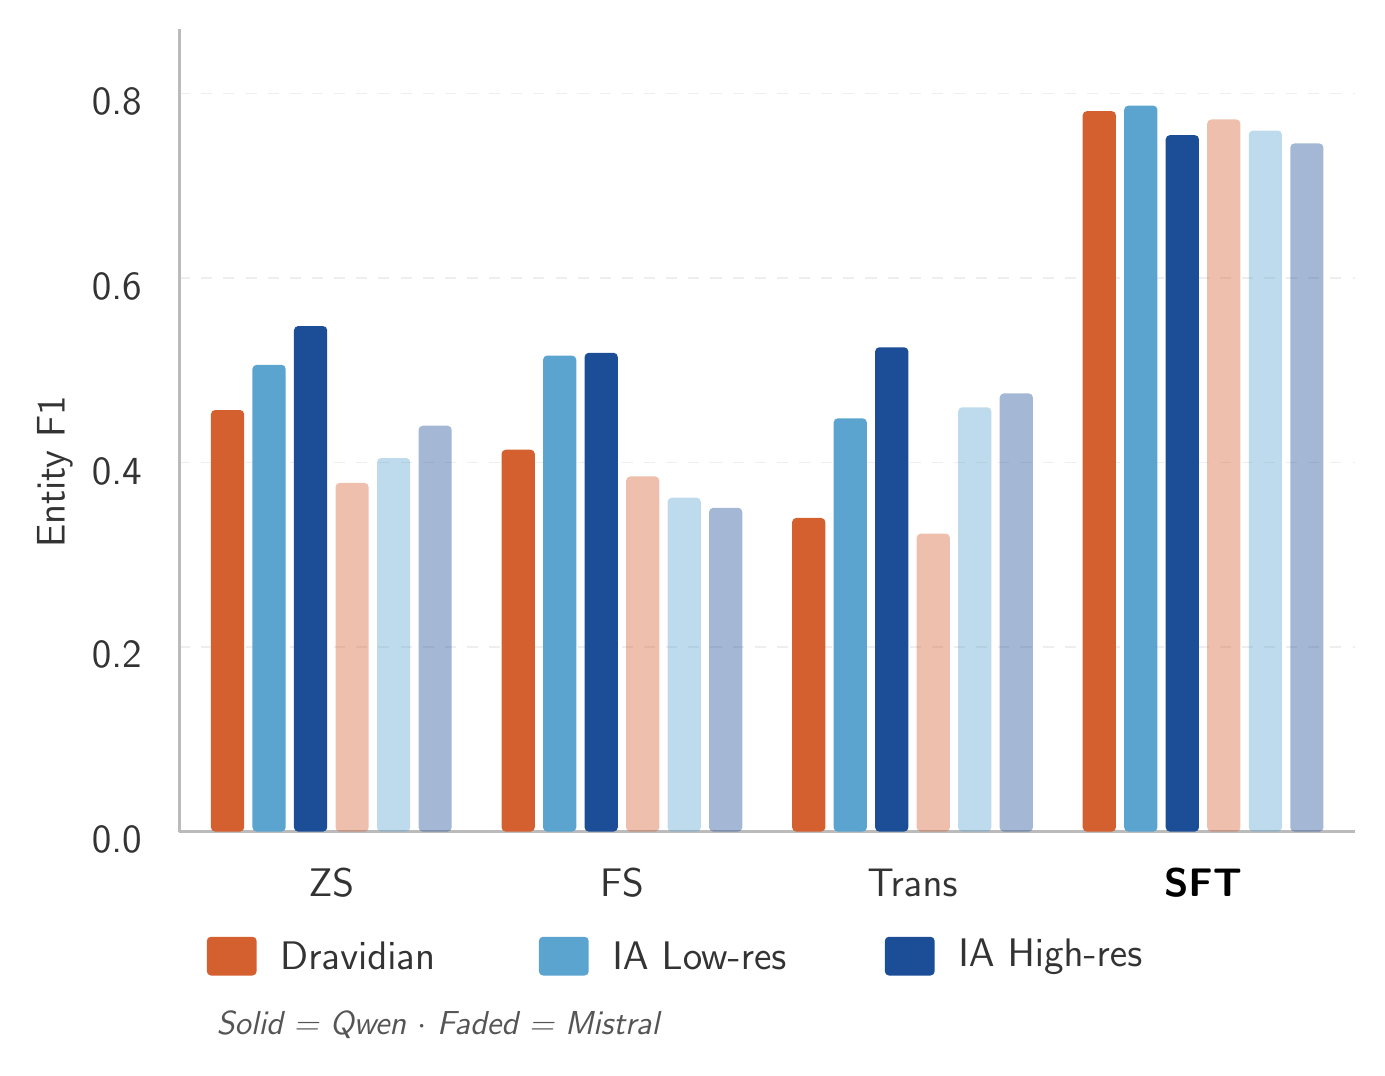
\begin{tikzpicture}[x=1pt, y=1pt]
    \foreach \ysvg/\yval in {233.3/0.2, 166.6/0.4, 100.0/0.6, 33.3/0.8}{
      \pgfmathsetmacro{\ytik}{300-\ysvg}
      \draw[gridcol, dash pattern=on 4pt off 4pt, line width=0.6pt]
        (55, \ytik) -- (480, \ytik);
    }
    \draw[axiscol, line width=1pt] (55, 0) -- (55, 290);
    \draw[axiscol, line width=1pt] (55, 0) -- (480, 0);
    \foreach \ysvg/\lbl in {303/0.0, 236/0.2, 170/0.4, 103/0.6, 36/0.8}{
      \pgfmathsetmacro{\ytik}{300-\ysvg}
      \node[anchor=east, font=\Large\sffamily, text=labelcol] at (45, \ytik) {\lbl};
    }
    \node[rotate=90, anchor=center, font=\Large\sffamily, text=labelcol] at (10, 130) {Entity F1};
    \newcommand{\drawbar}[4]{%
      \pgfmathsetmacro{\bh}{#2 * 333.333}%
      \fill[#3, opacity=#4, rounded corners=1.5pt] (#1, 0) rectangle (#1+12, \bh);%
    }
    % ZS
    \drawbar{66.5}{0.457}{colDrav}{1.0}
    \drawbar{81.5}{0.506}{colIAL}{1.0}
    \drawbar{96.5}{0.548}{colIAH}{1.0}
    \drawbar{111.5}{0.378}{colDrav}{0.4}
    \drawbar{126.5}{0.405}{colIAL}{0.4}
    \drawbar{141.5}{0.440}{colIAH}{0.4}
    % FS
    \drawbar{171.5}{0.414}{colDrav}{1.0}
    \drawbar{186.5}{0.516}{colIAL}{1.0}
    \drawbar{201.5}{0.519}{colIAH}{1.0}
    \drawbar{216.5}{0.385}{colDrav}{0.4}
    \drawbar{231.5}{0.362}{colIAL}{0.4}
    \drawbar{246.5}{0.351}{colIAH}{0.4}
    % Trans
    \drawbar{276.5}{0.340}{colDrav}{1.0}
    \drawbar{291.5}{0.448}{colIAL}{1.0}
    \drawbar{306.5}{0.525}{colIAH}{1.0}
    \drawbar{321.5}{0.323}{colDrav}{0.4}
    \drawbar{336.5}{0.460}{colIAL}{0.4}
    \drawbar{351.5}{0.475}{colIAH}{0.4}
    % SFT
    \drawbar{381.5}{0.781}{colDrav}{1.0}
    \drawbar{396.5}{0.787}{colIAL}{1.0}
    \drawbar{411.5}{0.755}{colIAH}{1.0}
    \drawbar{426.5}{0.772}{colDrav}{0.4}
    \drawbar{441.5}{0.760}{colIAL}{0.4}
    \drawbar{456.5}{0.746}{colIAH}{0.4}
    % X-axis labels
    \node[anchor=north, font=\Large\sffamily, text=labelcol] at (110, -10) {ZS};
    \node[anchor=north, font=\Large\sffamily, text=labelcol] at (215, -10) {FS};
    \node[anchor=north, font=\Large\sffamily, text=labelcol] at (320, -10) {Trans};
    \node[anchor=north, font=\Large\sffamily\bfseries, text=black] at (425, -10) {SFT};
    % Legend
    \fill[colDrav, rounded corners=1.5pt] (65,-52) rectangle (83,-38);
    \node[anchor=west, font=\Large\sffamily, text=labelcol] at (88, -45) {Dravidian};
    \fill[colIAL, rounded corners=1.5pt] (185,-52) rectangle (203,-38);
    \node[anchor=west, font=\Large\sffamily, text=labelcol] at (208, -45) {IA Low-res};
    \fill[colIAH, rounded corners=1.5pt] (310,-52) rectangle (328,-38);
    \node[anchor=west, font=\Large\sffamily, text=labelcol] at (333, -45) {IA High-res};
    \node[anchor=west, font=\large\sffamily\itshape, text=subtlecol] at (65, -70) {Solid = Qwen $\cdot$ Faded = Mistral};
    \end{tikzpicture}
    }
    \caption{Entity F1 by language family and condition. SFT narrows the Dravidian–Indo-Aryan gap from ${\sim}0.09$ to $<0.03$.}
    \label{fig:Entity_F1}
\end{figure}

\begin{table*}[t]
\centering
\caption{Macro-averaged results across all 10 languages. \best{Green bold}\,=\,best per row; \worst{red bold}\,=\,worst. For Hallucination and Omission, lower is better.}
\label{tab:macro_all_conditions}
\resizebox{\linewidth}{!}{%
\setlength{\tabcolsep}{5pt}
\begin{tabular}{lcccccccc}
\toprule
\textbf{Metric}
  & \textbf{Qwen ZS} & \textbf{Qwen FS} & \textbf{Qwen Trans} & \textbf{Qwen SFT}
  & \textbf{Mistral ZS} & \textbf{Mistral FS} & \textbf{Mistral Trans} & \textbf{Mistral SFT} \\
\midrule
Truthfulness
  & 3.318 & 3.370 & 2.811 & \best{4.156}
  & 3.092 & 3.067 & 2.777 & \best{4.084} \\
Safety
  & 2.560 & 2.575 & \worst{2.217} & 2.962
  & 2.496 & 2.354 & \worst{2.197} & 2.916 \\
Explainability
  & 3.388 & 3.302 & 2.676 & \best{3.838}
  & 3.052 & 2.932 & 2.716 & \best{3.828} \\
\midrule
ROUGE-L
  & 0.1318 & 0.1206 & 0.1478 & \best{0.2276}
  & 0.1352 & 0.1299 & 0.1476 & \best{0.2262} \\
BERTScore
  & 0.8557 & 0.8544 & 0.8501 & \best{0.8828}
  & 0.8478 & 0.8495 & 0.8501 & \best{0.8796} \\
\midrule
Precision
  & 0.5757 & 0.5418 & 0.4625 & \best{0.8946}
  & 0.4901 & 0.4437 & 0.4545 & \best{0.9021} \\
Hallucination\,$\downarrow$
  & 0.4243 & 0.4582 & \worst{0.5375} & \best{0.1054}
  & 0.5099 & 0.5563 & \worst{0.5455} & \best{0.0979} \\
Recall
  & 0.4837 & 0.4663 & 0.4359 & \best{0.6843}
  & 0.3917 & 0.3433 & 0.4012 & \best{0.6579} \\
Omission\,$\downarrow$
  & 0.5163 & 0.5337 & \worst{0.5641} & \best{0.3157}
  & 0.6083 & 0.6567 & \worst{0.5988} & \best{0.3421} \\
Entity F1
  & 0.5183 & 0.4992 & 0.4376 & \best{0.7745}
  & 0.4323 & 0.3852 & 0.4194 & \best{0.7604} \\
\bottomrule
\end{tabular}}
\end{table*}

\subsection{When In-Context Learning Fails}
\label{sec:fewshot}

The most striking finding in Table~\ref{tab:macro_all_conditions} is that
adding same-language demonstrations makes performance \emph{worse}, not
better, across most conditions.
Macro-average entity F1 falls from 0.518 to 0.499 for Qwen and from 0.432
to 0.385 for Mistral; hallucination rates rise by 3.4 and 4.6 percentage
points respectively.

We identify three mechanisms.
(1)~\textit{Template lock}: the demonstration summary encodes a particular
clinical narrative structure; the model adheres to it even when the test
dialogue contains content outside that structure.
Omission rates increase in 14 of 20 language--model combinations under
few-shot.
(2)~\textit{Entity bleed}: entities from demonstration dialogues (demographics,
medication names, symptom descriptions) migrate into the generated summary
for a different patient, inflating hallucination counts with clinically real but
contextually wrong content — an error invisible to surface-level metrics.
(3)~\textit{Calibration disruption}: for models already well-calibrated at
zero-shot, the demonstration introduces a competing prior.
The English condition illustrates this most clearly:
Mistral-English F1 drops from 0.652 to 0.558 under few-shot.

These observations are consistent with prior work showing that demonstrations
primarily encode format rather than semantic content~\cite{workrethinking},
and that few-shot biases hurt performance when the model's prior is already
reasonable~\cite{zhao2021calibrate}.
Two exceptions exist: Qwen-Gujarati (F1 $+0.134$) and Mistral-Telugu
(F1 $+0.096$), both of which have the highest zero-shot hallucination rates in
their respective matrices ($>0.69$).
Few-shot prompting is beneficial only when zero-shot generation is poor.

\subsection{Translation: A Typological Divide}

Table~\ref{tab:translation_vs_zs} shows the per-language impact of
translate-then-summarize.

\begin{table}[h!]
\centering
\caption{Translation vs.\ zero-shot entity F1 per language.}
\label{tab:translation_vs_zs}
\resizebox{\columnwidth}{!}{%
\begin{tabular}{llrrrr}
\toprule
\textbf{Lang.} & \textbf{Group}
  & \textbf{Q-ZS} & \textbf{Q-Tr}
  & \textbf{M-ZS} & \textbf{M-Tr} \\
\midrule
Hindi   & IA-High & .551 & \textcolor{bestgreen}{.571$\uparrow$} & .450 & \textcolor{bestgreen}{.561$\uparrow$} \\
Marathi & IA-Med  & .528 & \textcolor{bestgreen}{.635$\uparrow$} & .420 & \textcolor{bestgreen}{.570$\uparrow$} \\
Gujarati& IA-Low  & .394 & \textcolor{bestgreen}{.495$\uparrow$} & .368 & \textcolor{bestgreen}{.539$\uparrow$} \\
Dogri   & IA-Low  & .570 & .497$\downarrow$ & .431 & \textcolor{bestgreen}{.567$\uparrow$} \\
\midrule
\rowcolor{dravidianrow}
Telugu  & Drav. & .450 & \worst{.241$\downarrow$} & .282 & \worst{.200$\downarrow$} \\
\rowcolor{dravidianrow}
Tamil   & Drav. & .480 & .460$\downarrow$ & .429 & .473$\uparrow$ \\
\rowcolor{dravidianrow}
Kannada & Drav. & .441 & .319$\downarrow$ & .423 & \worst{.295$\downarrow$} \\
\midrule
Bengali & IA-High & .566 & \worst{.369$\downarrow$} & .451 & \worst{.295$\downarrow$} \\
Assamese& IA-Low  & .553 & \worst{.351$\downarrow$} & .417 & \worst{.275$\downarrow$} \\
\bottomrule
\end{tabular}}
\end{table}

For Indo-Aryan languages with Devanagari or closely related scripts,
translation consistently improves over zero-shot.
IndicTrans2 quality is high for these pairs, and structural proximity to Hindi
(the dominant Indic language in NMT training data) helps.
Mistral-Marathi gains 0.150 F1 and Mistral-Gujarati gains 0.171 — substantial
improvements for a training-free method.

For Dravidian languages, the outcome reverses sharply.
Qwen-Telugu drops 0.209 F1 under translation, with hallucination rising from
0.463 to 0.774.
Kannada and Tamil show similar degradation.
IndicTrans2 translation quality for Dravidian is substantially lower than for
Indo-Aryan: morphologically complex verb forms, clinical conditional structures,
and domain terminology are frequently mistranslated or collapsed.
The summarizer then operates on degraded input and cannot recover — a
\textit{mistranslation cascade}.
A single bad translation of a key clinical phrase (e.g., ``reduce tobacco use''
rendered as ``reduce their space'' in our Telugu case analysis) silently
eliminates content from the summary.

Bengali and Assamese also degrade despite not being Dravidian: IndicTrans2's
Bengali-trained model generalizes poorly to Assamese, and Bengali translation
hallucination nearly doubles (0.375 to 0.676). This warns against assuming
script family predicts translation quality; language-specific validation is
necessary before deployment.

Across all conditions, translation produces the lowest safety scores:
macro-averaged 2.217 (Qwen) and 2.197 (Mistral), with Mistral-Assamese
reaching 1.42/5.0. For Dravidian and low-resource languages, direct zero-shot
inference is safer than translation.

\subsection{Supervised Fine-Tuning Closes the Cross-Lingual Gap}
\label{sec:sft}

Table~\ref{tab:sft_gains} shows per-language SFT gains versus zero-shot.
Fine-tuning produces the strongest results across every metric, model, and
language.

The largest gains go to the languages that needed them most:
Mistral-Telugu $+0.487$, Qwen-Gujarati $+0.406$, Qwen-Kannada $+0.371$.
The Dravidian languages, which averaged F1 $\approx$ 0.457 (Qwen) and 0.378
(Mistral) at zero-shot, reach 0.781 and 0.772 post fine-tuning — nearly
identical to the high-resource Indo-Aryan group (0.756 and 0.747).
The cross-lingual performance gap is essentially eliminated: \emph{the gap is
not inherent to the languages but is an artifact of insufficient task-specific
training}.

Hallucination reductions are equally striking.
Macro-average hallucination drops from 42.4\% to 10.5\% for Qwen and from
50.9\% to 9.8\% for Mistral.
Mistral-Telugu, which hallucinated 71.8\% of entities at zero-shot, falls to
7.0\% post fine-tuning — below the English zero-shot rate of 29.6\%.

\begin{table}[h!]
\centering
\caption{SFT vs.\ zero-shot entity F1 per language. $\Delta$ = SFT $-$ ZS.}
\label{tab:sft_gains}
\resizebox{\columnwidth}{!}{%
\begin{tabular}{lrrrrrr}
\toprule
 & \multicolumn{3}{c}{\textbf{Qwen2.5-7B}} & \multicolumn{3}{c}{\textbf{Mistral-7B}} \\
\cmidrule(lr){2-4}\cmidrule(lr){5-7}
\textbf{Lang.} & ZS & SFT & $\Delta$ & ZS & SFT & $\Delta$ \\
\midrule
Bengali  & .566 & .720 & \textcolor{bestgreen}{+.154} & .451 & .708 & \textcolor{bestgreen}{+.257} \\
English  & .650 & .777 & \textcolor{bestgreen}{+.127} & .652 & .768 & \textcolor{bestgreen}{+.116} \\
Hindi    & .551 & .770 & \textcolor{bestgreen}{+.219} & .450 & .763 & \textcolor{bestgreen}{+.313} \\
Marathi  & .528 & .774 & \textcolor{bestgreen}{+.246} & .420 & .768 & \textcolor{bestgreen}{+.348} \\
\midrule
\rowcolor{dravidianrow}
Telugu   & .450 & \best{.808} & \textcolor{bestgreen}{+.358} & .282 & .769 & \textcolor{bestgreen}{+.487} \\
\rowcolor{dravidianrow}
Tamil    & .480 & .722 & \textcolor{bestgreen}{+.242} & .429 & .768 & \textcolor{bestgreen}{+.339} \\
\rowcolor{dravidianrow}
Kannada  & .441 & \best{.812} & \textcolor{bestgreen}{+.371} & .423 & .779 & \textcolor{bestgreen}{+.356} \\
\midrule
Gujarati & .394 & .800 & \textcolor{bestgreen}{+.406} & .368 & .769 & \textcolor{bestgreen}{+.400} \\
Dogri    & .570 & .776 & \textcolor{bestgreen}{+.206} & .431 & .757 & \textcolor{bestgreen}{+.326} \\
Assamese & .553 & .786 & \textcolor{bestgreen}{+.233} & .417 & .755 & \textcolor{bestgreen}{+.338} \\
\midrule
\textbf{Avg} & .518 & \textbf{.775} & \textbf{+.257} & .432 & \textbf{.760} & \textbf{+.328} \\
\bottomrule
\end{tabular}}
\end{table}

Despite these gains, neither model crosses 3.0/5.0 as a macro-average Safety
score even after fine-tuning.
The \emph{Truthfulness--Safety gap widens} under SFT: at zero-shot it is
$\approx$0.76 (Qwen) and 0.60 (Mistral); at SFT it grows to 1.19 and 1.17.
Models become more truthful much faster than they become safer.
This dissociation occurs because Safety penalizes not just factual errors but
also actionable omissions, inverted negations (``no dysphagia'' becoming
``mild dysphagia''), and conditionality collapse (``consider biopsy'' becoming
``biopsy is required'') — errors that supervised imitation of gold summaries
does not directly optimize against.
Safety-specific training signals, such as rubric-grounded reward models or
reinforcement learning from clinical expert feedback, are likely necessary.

\subsection{Qwen vs.\ Mistral}

At zero-shot, Qwen2.5-7B leads Mistral-7B on every entity-level metric: F1
0.518 vs.\ 0.432 ($+$0.086), precision 0.576 vs.\ 0.490, hallucination rate
0.424 vs.\ 0.510, Truthfulness margin $+$0.226, Explainability margin $+$0.336.
Qwen's advantage traces to its broader multilingual pretraining: token
representations for non-Latin scripts are better calibrated across Dravidian
and low-resource Indo-Aryan languages.
After fine-tuning the gap narrows to F1 0.775 vs.\ 0.760 ($+$0.014).
Practitioners should prefer Qwen2.5-7B for prompting-based deployment; for
fine-tuned deployment, both models are viable.

% ==================================================================
\section{Clinical Error Taxonomy}
\label{sec:CET}

Through systematic qualitative analysis across all ten languages, we identified
eight recurring failure mechanisms, organized into the Clinical Error Taxonomy
in Table~\ref{tab:error_taxonomy}.

\begin{table}[h!]
\centering
\small
\caption{Eight-category Clinical Error Taxonomy.}
\label{tab:error_taxonomy}
\begin{tabularx}{\columnwidth}{l >{\raggedright\arraybackslash}p{1.8cm} X}
\toprule
\textbf{ID} & \textbf{Error Type} & \textbf{Description \& Context} \\
\midrule
\textbf{T1} & Temporal Distortion & Numerals extract correctly but units are substituted (e.g., ``3 months'' $\to$ ``3 days''). Low-resource ZS. \\
\addlinespace
\textbf{T2} & Pathology Fabrication & Clinically plausible but invented diagnoses (e.g., ``apnea'' for throat pain). Dravidian ZS. \\
\addlinespace
\textbf{T3} & Entity Bleed & Valid entities from demonstration examples migrate to the test patient. Few-shot. \\
\addlinespace
\textbf{T4} & Frequency Inversion & Substance use frequencies minimized (e.g., ``3–4x/week'' $\to$ ``occasional''), skewing risk stratification. All paradigms. \\
\addlinespace
\textbf{T5} & Conditionality Collapse & Conditional plans rendered as definitive (e.g., ``consider biopsy'' $\to$ ``biopsy required''). FS \& Trans. \\
\addlinespace
\textbf{T6} & Speaker Misattribution & Physician advice attributed to patient. NMT drops Dravidian grammatical honorifics. \\
\addlinespace
\textbf{T7} & Fabricated Absence & False hedging (e.g., ``no side effects reported'') masking missing extractions. Translation. \\
\addlinespace
\textbf{T8} & Mistranslation Cascade & NMT error yields semantically empty English, silently eliminating crucial content. Severe in Dravidian/Assamese. \\
\bottomrule
\end{tabularx}
\end{table}

% ==================================================================
\section{Human Evaluation}

To validate our LLM-as-judge evaluation, we conducted a human study across
four languages (Tamil, Kannada, Marathi, Hindi).
Annotators evaluated zero-shot and few-shot summaries using the same
three-dimensional rubric (Truthfulness, Safety, Explainability) plus an
overall trust rating.
Human annotations corroborate the automated findings: while few-shot prompting
often improves superficial flow and formatting (higher Explainability scores),
it actively introduces clinical hallucinations — e.g., fabricating geographic
locations such as ``Pune'' not mentioned in any dialogue — and degrades
factual Truthfulness.

% ==================================================================
\section{Discussion}

Our results expose a quantified reliability gap in multilingual clinical AI.
Dravidian language users face hallucination rates roughly 15 percentage points
higher than English users at zero-shot.
Translation amplifies this gap rather than narrowing it.
Few-shot prompting degrades performance even with same-language demonstrations,
ruling out cross-lingual interference as the sole explanation.
Fine-tuning on domain-matched multilingual data is the \emph{only} strategy
that closes the gap.
Deploying English-optimized clinical LLMs without fine-tuning produces
documentation that is measurably less safe for Dravidian-language speakers.

The entity-bleed mechanism is specific to domain-homogeneous settings where
demonstration and test dialogues share a clinical context: entities transfer
plausibly but incorrectly.
This is a warning for any high-stakes domain using in-domain few-shot examples.

The persistent safety deficit after SFT points to a training objective gap.
Imitating gold summaries optimizes truthfulness but does not penalize dangerous
omissions, inverted negations, or conditionality collapse.
Safety-specific reward models or expert feedback loops are likely necessary
to close this gap.
The AI-ML systems research agenda should prioritize infrastructure for
safety-aware multilingual fine-tuning: rubric-grounded reward models,
language-stratified evaluation pipelines, and translation quality gating
before summarization.

% ==================================================================
\section{Conclusion}

We present the first systematic evaluation of cross-lingual clinical dialogue
summarization across ten Indian languages.
Few-shot prompting consistently degrades performance through template lock,
entity bleed, and calibration disruption.
Translation via IndicTrans2 helps Indo-Aryan languages but harms Dravidian
and low-resource languages through mistranslation cascades.
Clinical Safety scores remain below 3.0/5.0 across all conditions and both
models, even after fine-tuning.
Supervised fine-tuning closes the cross-lingual gap:
Kannada and Telugu reach entity F1 scores competitive with English.
Safety evaluations conducted only in English systematically underestimate the
clinical risk faced by speakers of low-resource languages;
evaluation frameworks must reflect this linguistic reality.

% ==================================================================
\bibliographystyle{IEEEtran}
\bibliography{aimlsystems2026}

\end{document}
